\documentclass[12pt]{article}
\everymath{\displaystyle}
\usepackage{unicode-math}
\usepackage{pgfplots}
\pgfplotsset{compat=1.18}
\usepackage{amsmath}



\usepackage[margin=1in]{geometry}
\usepackage{tcolorbox}
\usepackage{graphicx}
\usepackage{tikz}
\usepackage{amssymb}
\usepackage{enumitem}
\usepackage{titlesec}
\usepackage{fancyhdr}
\usepackage{pifont}
\usepackage{xcolor}
\newcounter{questionnum}
\setcounter{questionnum}{0}
\usepackage{eso-pic} % for page background

% --------- 主题颜色设置 ---------
\definecolor{novelblue}{RGB}{70,60,150}
\definecolor{headerbg}{RGB}{240,240,255}

\pagestyle{fancy}
\fancyhf{}
\renewcommand{\headrulewidth}{0.4pt}
\renewcommand{\headrule}{\hbox to\headwidth{\color{novelblue}\leaders\hrule height 0.4pt\hfill}}

% --------- 页眉背景色条 ---------
\newcommand{\headbackground}{
  \AddToShipoutPictureBG*{
    \begin{tikzpicture}[remember picture, overlay]
      \fill[blue!5!purple!10] (current page.north west) rectangle ([yshift=-60pt]current page.north east);
    \end{tikzpicture}
  }
}

% --------- 页眉设置 ---------
\pagestyle{fancy}
\fancyhf{}
\renewcommand{\headrulewidth}{0pt}
\fancyhead[L]{\color{novelblue}\textbf{\textbf{Novel Prep} }}
\fancyhead[C]{\color{novelblue}\textbf {SAT Preparation}}
\fancyhead[R]{\color{novelblue}\textbf{Jack Zeng}}


\newtcolorbox{SATCard}[1][]{%
  enhanced,
  colback=white,
  colframe=novelblue,
  coltitle=white,
  boxrule=0.6pt,
  arc=4pt,
  boxsep=5pt,
  left=8pt, right=8pt, top=10pt, bottom=10pt,
  sharp corners=south,
  drop shadow south east,
  #1
}

% --------- 顶部 Mark for Review 栏 ---------
\newcommand{\markforreview}{
  \stepcounter{questionnum} % 自动递增题号
  \begin{tikzpicture}[scale=1.1]
    % 黑色题号
    \fill[black] (0,0) rectangle (0.8,0.6);
    \node[white, font=\bfseries\large] at (0.4,0.3) {\thequestionnum};

    % 灰底主栏
    \fill[gray!10] (0.8,0) rectangle (14.5,0.6);

    % Mark for Review
    \node[anchor=west, font=\small] at (1.2,0.3) {\ding{72} \hspace{2pt}Mark for Review};

    % ABC 按钮区域
    \draw[thick, rounded corners=3pt] (13.5,0.12) rectangle (14.5,0.48);
    \node[font=\bfseries\normalsize] at (14.0,0.3) {ABC};
  \end{tikzpicture}


  \newcommand{\choiceboxcircled}[2]{%
  \begin{tcolorbox}[
    colback=white,
    colframe=black,
    boxrule=0.5pt,
    rounded corners=6pt,
    left=6pt, right=6pt, top=6pt, bottom=6pt,
    width=\linewidth
  ]
    \textbf{\large\textcircled{\textbf{#1}}} \ #2
  \end{tcolorbox}
}
}

% --------- 选项框样式 ---------
\newcommand{\choicebox}[2]{%
  \begin{tcolorbox}[
    colback=white, 
    colframe=novelblue,
    boxrule=0.5pt, 
    rounded corners=4pt, 
    left=6pt, right=6pt, top=6pt, bottom=6pt,
    width=\linewidth
  ]
  \textbf{#1.} \ #2
  \end{tcolorbox}
}


\begin{document}


\section*{SAT Linear Equation Practice}

\noindent\markforreview
\vspace{1em}

For each real number \(r\), which of the following points lies on the graph of both equations in the \(xy\)-plane for the given system?

\[
\begin{aligned}
15x + 45y &= 33 \\
5x + 15y &= 11
\end{aligned}
\]

\choicebox{A}{\(\left( \frac{11r}{5} - 3, r \right)\)}  
\choicebox{B}{\(\left( -3r + \frac{11}{5}, r \right)\)}  
\choicebox{C}{\(\left( r, -\frac{r}{3} - \frac{11}{15} \right)\)}  
\choicebox{D}{\(\left( r, \frac{r}{3} + \frac{11}{15} \right)\)}

\vspace{2em}

\newpage
\noindent\markforreview
\vspace{1em}

The given equation is one equation in a system of two linear equations.  
If the system has at least one solution, which of the following equations could be the other equation in the system?  
\[
7x + 5y = 2
\]

\noindent I. \(10.5x + 7.5y = 3\)  

\noindent II. \(10.5x - 7.5y = 3\)

\choicebox{A}{I only}  
\choicebox{B}{II only}  
\choicebox{C}{I and II}  
\choicebox{D}{Neither I nor II}

\vspace{2em}

\newpage
\noindent\markforreview


\begin{center}
    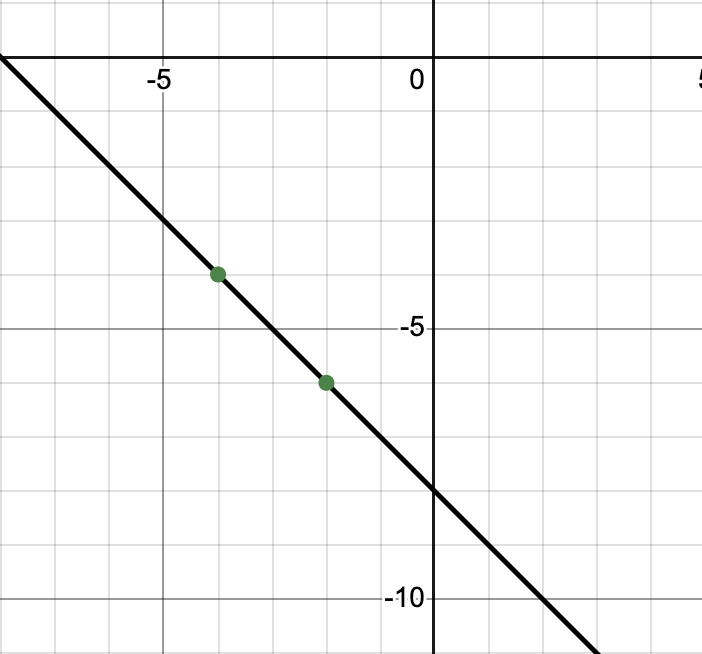
\includegraphics[width=0.4\linewidth]{f10.png}
\end{center}

The graph of the linear function \( y = f(x) - 19 \) is shown.  
If \(c\) and \(d\) are positive constants, which equation could define \(f\)?

\choicebox{A}{\(f(x) = d - cx\)}  
\choicebox{B}{\(f(x) = -d + cx\)}  
\choicebox{C}{\(f(x) = d + cx\)}  
\choicebox{D}{\(f(x) = -d - cx\)}

\vspace{2em}

\newpage
\noindent\markforreview
\vspace{1em}

A beekeeper’s initial observation of the population of a certain bee colony was 1,100 bees.  
The beekeeper set a goal to increase the population to 2,600 bees.  

The beekeeper uses a model that predicts the population of this bee colony:
\begin{itemize}
\item begins at 1,100  
\item increases by 120 bees per week in the first two weeks  
\item then increases by 180 bees per week until the goal is reached  
\end{itemize}

According to this model, at the end of week \(w\) after the initial observation, where \(w > 2\),  
which of the following functions gives the predicted number of bees still needed to reach the beekeeper’s goal?

\choicebox{A}{\(p(w) = 2600 - 180w\)}  
\choicebox{B}{\(p(w) = 2480 + 180w\)}  
\choicebox{C}{\(p(w) = 1620 - 180w\)}  
\choicebox{D}{\(p(w) = -120 + 180w\)}

\vspace{2em}

\newpage
\noindent\markforreview
\vspace{1em}

The table shows three values of $x$ and their corresponding values of $y$, where $s$ is a constant. There is a linear relationship between $x$ and $y$. Which of the following equations represents this relationship?

\[
\begin{array}{|c|c|}
\hline
x & y \\
\hline
-2s & 24 \\
-s & 21 \\
s & 15 \\
\hline
\end{array}
\]

\choicebox{A}{$sx + 3y = 18s$}  
\choicebox{B}{$3x + sy = 18s$}  
\choicebox{C}{$3x + sy = 18$}  
\choicebox{D}{$sx + 3y = 18$}



\vspace{2em}
\newpage

\noindent\markforreview
\vspace{1em}

The table shows three values of $x$ and their corresponding values of $g(x)$, where 
\[
g(x) = \frac{f(x)}{x + 5}
\]
and $f$ is a linear function. What is the $y$-intercept of the graph of $y = f(x)$ in the $xy$-plane?

\[
\begin{array}{|c|c|}
\hline
x & g(x) \\
\hline
-20 & 4 \\
-8 & 0 \\
10 & 6 \\
\hline
\end{array}
\]

\choicebox{A}{$(0, -8)$}  
\choicebox{B}{$(0, 5)$}  
\choicebox{C}{$(0, 8)$}  
\choicebox{D}{$(0, 40)$}

\newpage
\noindent\markforreview
\vspace{1em}

    \begin{center}
        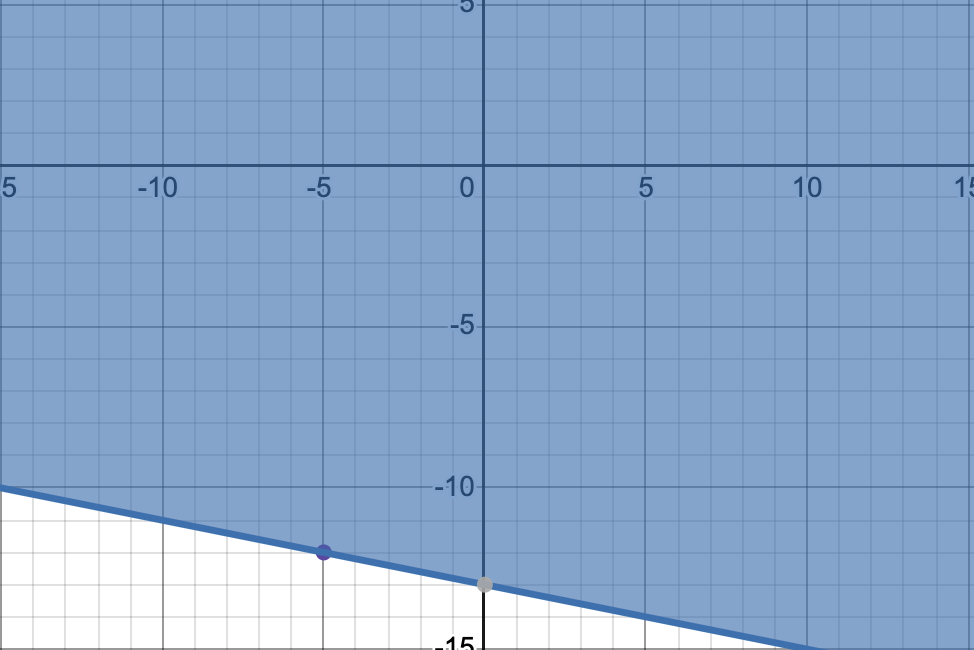
\includegraphics[width=0.6\linewidth]{f7.png}
    \end{center}


The shaded region represents the solutions to the inequality:  
\[
rx + ty \geq -65
\]  
What is the value of \(r + t\)?

\choicebox{A}{6}  
\choicebox{B}{4}  
\choicebox{C}{-4}  
\choicebox{D}{-5}

\vspace{2em}
\newpage
\noindent\markforreview
\vspace{1em}

Keenan made 32 cups of vegetable broth. Keenan then filled $x$ small jars and $y$ large jars with all the vegetable broth he made. The equation $3x + 5y = 32$ represents this situation. 

What is the best interpretation of $5y$ in this context?

\choicebox{A}{The number of large jars Keenan filled}  
\choicebox{B}{The number of small jars Keenan filled}  
\choicebox{C}{The total number of cups of vegetable broth in the large jars}  
\choicebox{D}{The total number of cups of vegetable broth in the small jars}

\vspace{2em}


\noindent\markforreview
\vspace{1em}

One gallon of stain will cover 170 square feet of a surface. A yard has a total fence area of $w$ square feet.

Which equation represents the total amount of stain $S$, in gallons, needed to stain the fence in this yard \textbf{twice}?

\choicebox{A}{$S = \dfrac{w}{170}$}  
\choicebox{B}{$S = 170w$}  
\choicebox{C}{$S = 340w$}  
\choicebox{D}{$S = \dfrac{w}{85}$}

\vspace{2em}







\end{document}